%----------------------------------------------------------------------------------------
%	FORMATION EARLY SOLAR SYSTEM.
%----------------------------------------------------------------------------------------
\section{The formation of comets and asteroids in the early solar system}
\subsection{Creation of asteroids and comets and their H/D Ratio}
\subsubsection{Creation of asteroids}
In the Solar System, there are two main sources for asteroids and comets: the asteroid belt and the Kuiper Belt. The former is located between the terrestrial planets and the gas planets in a region that is often referred to as the snow line \cite{asteroid_belts}, while the latter is located further out than any of the known planets.

In the early states of the solar system, asteroids in the asteroid belt formed within the solar nebula. This process would not differ from the formation of the other planets were it not for the presence of Jupiter, the closest gas giant to the snow line. The gravitational forces and disturbances prevent the small planetesimals to form a planet. In addition to this, these disturbances could cause the asteroids to leave the asteroid belt and collide with other bodies in the solar system. \cite{asteroid_belts}

\subsubsection{Creation of comets}
In the present solar system the comets encountered in the inner solar system usually originate from either the Kuiper Belt or the Oort cloud. However, it is likely that the comets were not originally formed there.
For the formation of comets there are two plausible locations: either in the neighborhood of Uranus and Neptune or further out where the temperature was lower and the gravitational forces not as disturbing as in the vicinity of Uranus and Neptune. The low-density environment of the Oort cloud would not provide enough particles for the comets to form, so it is suggested that comets found in this region were formed somewhere else and then ejected into the Oort cloud.
If comets were formed near Uranus and Neptune the comets would probably be absorbed by the planets or ejected onto hyperbolic trajectories rather than just being ejected into larger-distance orbits within the Oort cloud \cite{comets_radiation_pressure}. This leaves the most likely point of formation outside the orbits of Neptune and Jupiter \cite{comets_origin}.


\subsection{Water distribution in the early states of the solar system and contribution to the formation of asteroids and comets}

The early states of the Solar System with its hot inner core near the proto sun have mainly contributed to the fact that the only water-rich asteroids originally came from the outer asteroid belt and the Kuiper Belt. Up to 10 percent of their mass is water \cite{timescale}. 

The possible areas where water particles can aggregate and therefore be found in bodies such as asteroids and comets as well as planets and planetary satellites are beyond the snow line that marks the area where H\textsubscript{2}O only occurs as water ice and not as water particles or water vapor. Figure \ref{fig::lifetimes_ice_grains} shows the expected lifetime of pure and dirty ice grains depending on the grain size \cite{snow_line_age}.

\begin{figure}
	\centering
	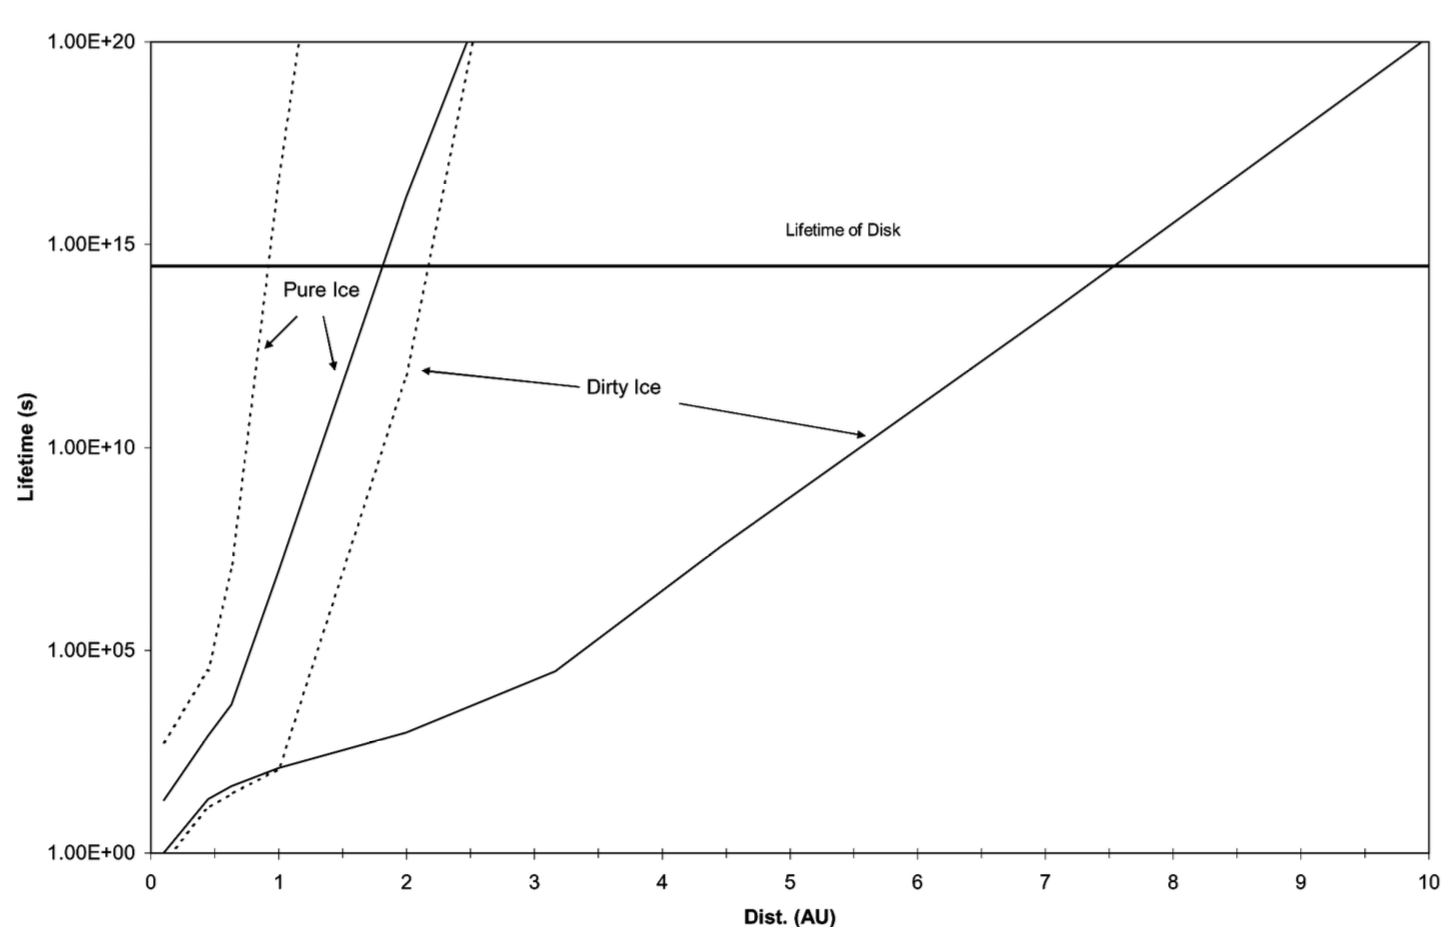
\includegraphics[width=0.7\textwidth]{figures/lifetime_water_ice}
	\caption{Comparison of lifetimes for pure and dirty ice grains. The dashed curves are for 0.1 $\mu$m grains and the solid curves are for 10 $\mu$m grains. The solid horizontal line shows a conservative upper limit to the age of the gas disk.  \cite{snow_line_age}}
	\label{fig::lifetimes_ice_grains}
\end{figure}


\subsection{H/D ratio in comets and asteroids}

The D/H ratio in comets and asteroids is linked to their formation region and therefore differs for various asteroids as well as comets from the Oort cloud and the Kuiper Belt and can be related to the D/H ratio in the solar nebula and the different planets. 
An overview of measured and estimated data is given in Figure \ref{fig::D_H_ratio_solar_system}

%\begin{figure}
%	\centering
%	\includegraphics[width=0.9\textwidth]{figures/D_H_ratio_outer_solar_system}
%	\caption{D/H ratios of various objects in the solar system.  \cite{constraints_comets_dhratio}}
%	\label{fig::D_H_ratio_outer_solar_system}
%\end{figure}

\begin{figure}
	\centering
	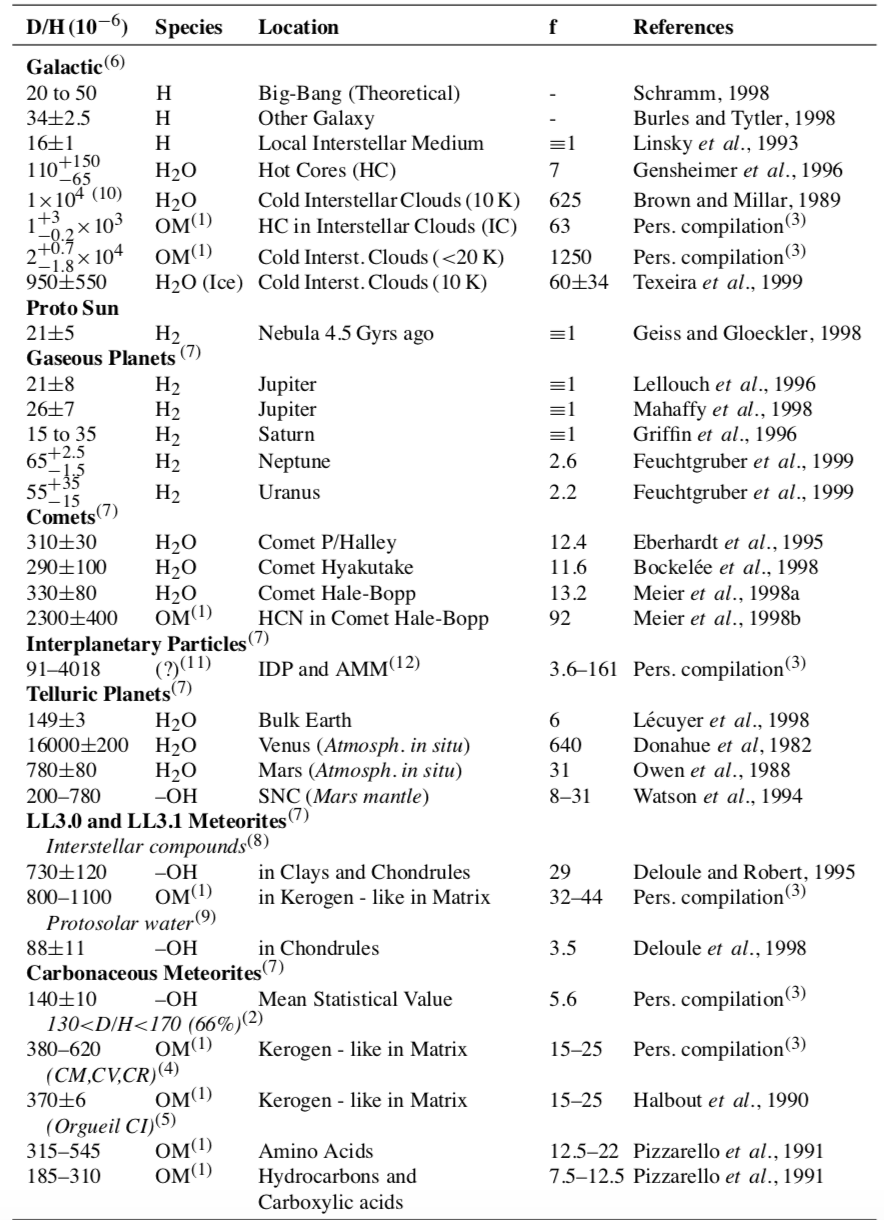
\includegraphics[width=0.9\textwidth]{figures/D_H_ratio_solar_system}
	\caption{D/H ratios of various objects in the solar system.  \cite{SolSystemDH_Robert}}
	\label{fig::D_H_ratio_solar_system}
\end{figure}

However, more recent observations of comet 103P/Hartley 2 have shown that it's H/D ratio is $(161 \pm 24) \times 10^{-6}$ and therefore significantly lower than estimated from previous measurements of other comets. This could be the case because the origin of 103P/Hartley 2 is not known for a certainty but it is believed that it could have originated in the Kuiper Belt, contrarily to a lot of other comets such as 1P/Halley who are widely believed to have originated in the Oort cloud. \cite{water_Hartley2_nature}

For comets it has been suggested that the deuterium enrichment factor depends on the creation epoch of the comet which is different for Kuiper Belt comets and comets from the Oort cloud, due to different temperature scales and depends on the evolution of the solar nebula over time. 

Using the enrichment factor $f$ for water
\begin{equation}
	f = \frac{1/2}{1/2} \frac{HDO/H_2O}{HD/H_2}
\end{equation}
which quantifies the D/H ratio for a certain deuteriated species, in this case water. As mentioned above, the deuterium enrichment factor $f$ depends on the temperature distribution of the isotopic exchange as well as the pressure distribution which is also temperature-dependent. The differential equation is given in Equation \ref{equ::diff_equ_f} \cite{transport_solar_nebula}:

\begin{equation}
	\partial_t f = \underbrace{k(T) P(A(T) - f)}_{\textrm{diffusion term}} + \underbrace{\frac{1}{\Sigma R} \partial_R (\kappa R \Sigma\partial_R f)}_{\textrm{exchange term}}
	\label{equ::diff_equ_f}
\end{equation}
$A(T)$ is the fractation at equilibrium, $P$ is the total pressure $R$ is the heliocentric distance, $k(T)$ is the isotopic exchange, $\Sigma$ is the gas surface density and $\kappa$ describes the turbulent diffusivity which depends on the nature of the turbulence. Equation \ref{equ::diff_equ_f} can be split up in an exchange and a diffusion term, the former describes the dependency of the heliocentric distance while the latter describes the dependency on the temperature distribution.

This connection is displayed and compared with measurement data from various comets in Figure \ref{fig::D/H_distance_age}.

\begin{figure}
	\centering
	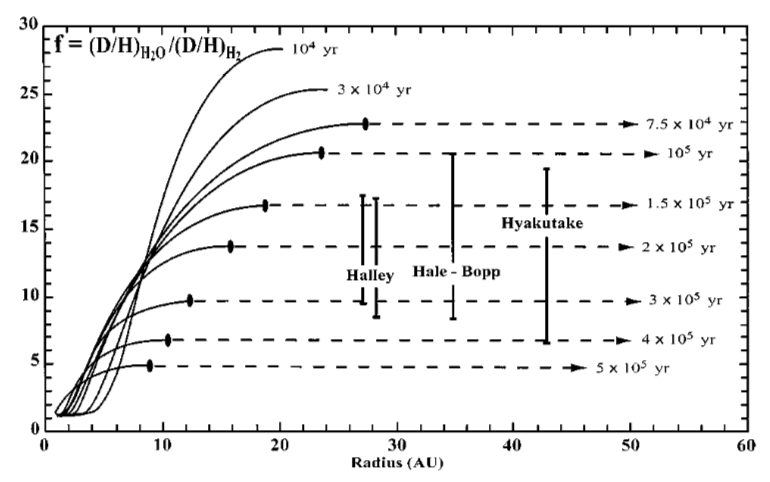
\includegraphics[width=0.5\textwidth]{figures/D_H_distance_time}
	\caption{Calculated deuterium enrichment factor f in H2O as a function of the heliocentric distance R, at various epochs in years of the evolution of the nebula. Dots indicate the heliocentric distance where H2O condenses. Dashed lines correspond to the value of f in ices. D/H enrichments obtained in comets Halley, Hyakutake, and Hale–Bopp are shown for comparison. The location of comets is arbitrary.  \cite{constraints_comets_dhratio}}
	\label{fig::D/H_distance_age}
\end{figure}


Meteorites with high D/H ratio are only those of the following two types: LL3 and carbonaceous chondrites. In both types, the insoluble organic matter shows elevated values of deuterium enrichment as well as clay minerals. The values obtained from the measurements of clay minerals can then be used to determine the D/H ratio of water because of the negligible isotopic fractionation between clay minerals and liquid water. \cite{SolSystemDH_Robert}


\newpage
\subsection{Measurement data from 67P/Churyumov-Gerasimenko}
67P/Churyumov-Gerasimenko is a Jupiter-family comet that probably originated in the Kuiper Belt. During the Rosetta Mission detailed measurements of the D/H ratio were conducted, resulting in a D/H ratio of $(530 \pm 70)\times10^{-6}$, 3 times higher than the values found on Earth. Although 67P/Churyumov-Gerasimenko is expected to come from the same region of the Solar System as 103P/Hartley 2 (discussed in the previous section), they show significantly different values that suggest that the variety of Jupiter-family comets is greater than expected.  

\begin{figure}
	\centering
	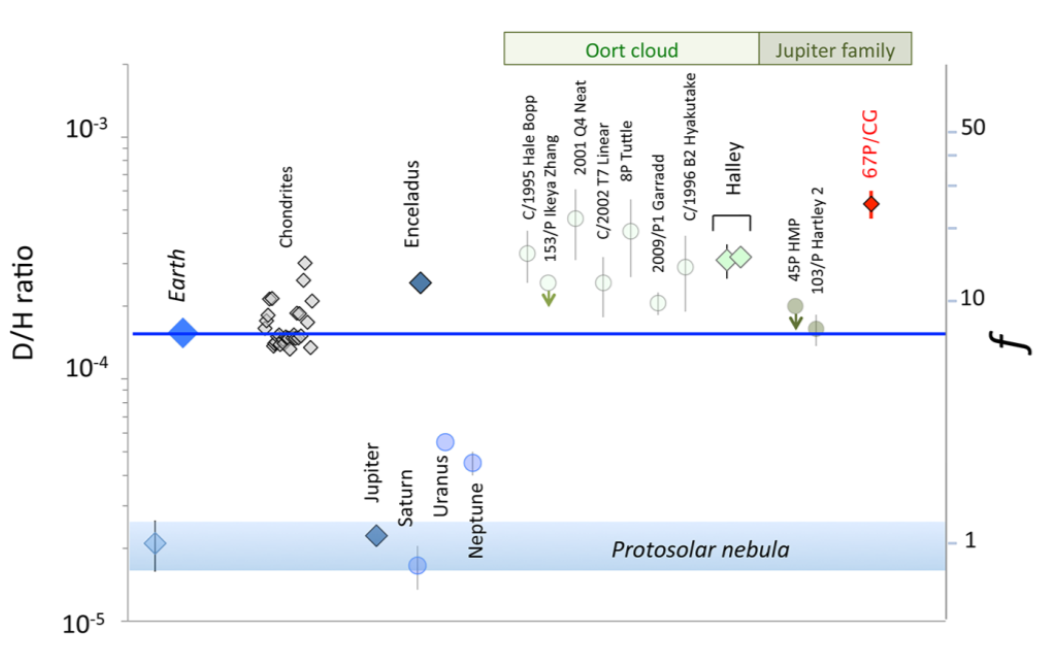
\includegraphics[width=0.6\textwidth]{figures/D_H_ratio_multiple_objects}
	\caption{D/H ratios in different objects of the solar system. Diamonds represent data obtained by in-situ mass spectrometry measurements, and circles refer to data obtained by astronomical methods. \cite{D/H_67P_science}}
	\label{fig::D/H_different_objects}
\end{figure}

